


\chapter{The Near-Earth Environment}
  \label{ch_environment}

%ALEX NOTES
%## Chapter 2
%### 2.1
%- I'm not sure what "width" and "length" means when measuring a magnetosphere.
%- I wonder if I have any relation to this Dungey... That's my mother's maiden
%  name.
%### 2.2
%- I think standard practice is to use em dashes without spaces.

From Earth's surface to a height of a hundred kilometers or so, the atmosphere
is a well-behaved fluid: a collisional ensemble of neutral atoms. Higher up,
its behavior changes dramatically. As altitude increases, solar ultraviolet
radiation becomes more intense, which ionizes atmospheric atoms and molecules.
Density also decreases, slowing collisional recombination. Whereas the neutral
atmosphere is held against Earth's surface by gravity, the motion of charged
particles is dominated by Earth's geomagnetic field, as well as the
electromagnetic disturbances created as that field is hammered by the solar
wind. 

Before discussing specific interactions, it's appropriate to introduce the
so-called ``frozen-in condition.'' In a collisionless plasma, magnetic field
lines are equiputential contours. Charged particles move freely along the
contours, but cannot move across them. Compression of the magnetic field is
synonymous with compression of the ambient plasma, as any magnetic field lines
that thread a moving plasma are dragged along with it. This assumption is valid
throughout most of the magnetosphere --- that is, the region of space primarily
governed by Earth's magnetic field --- and provides an invaluable tool for
understanding the large-scale motions of plasmas and fields. 

%\todo{Neutral density is larger than charged particle density (?) but it doesn't matter because mean free path is huge. }

% -----------------------------------------------------------------------------
% -----------------------------------------------------------------------------
% -----------------------------------------------------------------------------
\section{The Outer Magnetosphere}
  \label{sec_outer}

%\footnote{In the case of an ideal plasma, \ohmlaw takes the form $\vec{E} + \vec{U} \times \vec{B} = 0$. }. 

%\todo{Jets from magnetic reconnection... release of magnetic tension! }

Plasma behavior within Earth's magnetosphere is ultimately driven by the solar
wind: a hot (\about\SI{100}{\eV}), fast-moving (\about\SI{100}{\km/\s}) plasma
threaded by the interplanetary magnetic field
(\about\SI{10}{\nT})\footnote{Listed values correspond to the solar wind at
Earth's orbit. }. The density of the solar wind is on the order of
\SI{10}{\percc}; in a laboratory setting, this would constitute an ultra-high
vacuum (atmospheric density at sea level is \about\SI{e19}{\percc}), but
compared to much of the magnetopause it's quite dense. 

\begin{figure}[!htb]
  \centering
  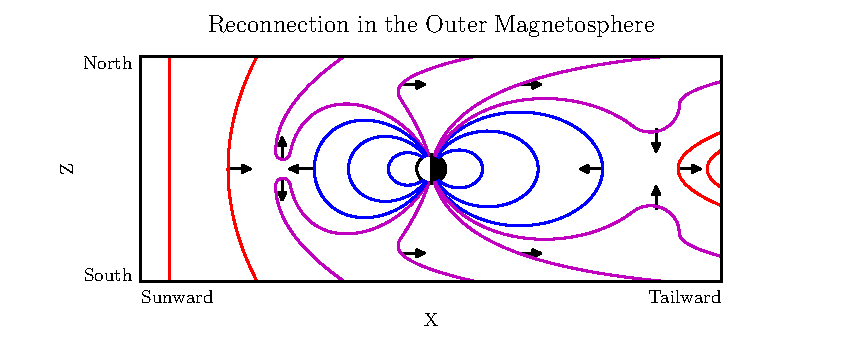
\includegraphics[width=\textwidth]{figures/outer_magnetosphere.pdf}
  \caption[Reconnection in the Outer Magnetosphere]{
    When the solar wind magnetic field (red) points southward, reconnection can
    occur between it and Earth's (northward) closed magnetic field lines
    (blue). The resulting open field lines (magenta) convect nightward over the
    poles, ultimately arriving in the magnetotail. There, the open field lines
    reconnect again. Newly closed field lines move Earthward, carrying flux
    across the flanks and back to the dayside. The rest are completely
    decoupled from Earth, and are lost to the solar wind. 
  }
  \label{fig_outer_magnetosphere}
\end{figure}

The magnetosphere's outer boundary represents a balance between the solar wind
dynamic pressure and the magnetic pressure of Earth's dipole field. On the
dayside, the dipole is compressed, pushing this boundary to within about
\SI{10}{\RE} of Earth\footnote{Distances in the magnetosphere are typically
measured in units of Earth radii: $\SI{1}{\RE} \equiv \SI{6378}{\km}$. }. The
nightside magnetosphere is stretched into a long tail which may exceed
\SI{50}{\RE} in width and \SI{100}{\RE} in length. 

When the interplanetary magnetic field opposes the geomagnetic field at the
nose of the magnetosphere, magnetic reconnection occurs. Closed magnetospheric
field lines ``break,'' opening up to the interplanetary magnetic
field\footnote{Closed field lines are more or less dipolar; one end connects to
the north pole of Earth's magnetic core, and the other end to the south pole.
Open field lines are tethered to Earth at one end. In principle, the other end
eventually doubles back to Earth, but for practical purposes it is lost to the
solar wind. The distinction is important because charged particle motion is
guided by magnetic field lines, as discussed in \cref{ch_flrs}. }. They then
move tailward across the poles, dragging their frozen-in plasma with them.
Reconnection in the tail allows magnetic field lines to convect back to the day
side, across the flanks. This process is called the Dungey
cycle\cite{dungey_1961}. 

Viewed from the north, the Dungey cycle involves a clockwise flow of flux and
plasma on the dusk side and a counterclockwise flow on the dusk side. The
motion is accompanied by a convection electric field, per \ohmlaw in an ideal
plasma:
\begin{align}
  \vec{E} + \vec{U} \times \vec{B} = 0
\end{align}

Where \vec{B}, \vec{E}, and \vec{U} are the magnetic field, electric field, and
plasma velocity vectors respectively. 

Consistent with \amplaw, the interplanetary magnetic field is separated from
the magnetosphere by a current sheet: the magnetopause. On the dayside, the
magnetopause current flows duskward; on the nightside, it flows dawnward around
the magnetotail. 

Earth's dipole is significantly deformed in the magnetotail; field lines in the
northern lobe of the tail points more or less Earthward, and vice versa. Plasma
within the lobes is cool (\about\SI{100}{\eV}) and rarefied
(\about\SI{e-2}{\percc}). The two lobes are divided by the plasma sheet, which
is comparably hot (\about\SI{e3}{\eV}) and dense (\about\SI{1}{\percc}). The
plasma sheet carries a duskward current which connects to the magnetopause
current. 

% -----------------------------------------------------------------------------
% -----------------------------------------------------------------------------
% -----------------------------------------------------------------------------
\section{The Inner Magnetosphere}

Within $L \sim 8$ (where $L$ is the McIlwain parameter\footnote{The McIlwain
parameter $L$ is used to index field lines in Earth's dipole geometry:
$L \equiv \frac{r}{\sin^2\theta}$ for colatitude $\theta$ and radius $r$ in
Earth radii. For example, the $L=5$ field line passes through the equatorial
plane at a geocentric radius of \SI{5}{\RE}, then meets the Earth at a
colatitude of $\arcsin \sqrt{ \frac{1}{5} } \sim \SI{27}{\degree}$ (equally, a
latitude of $\arccos \sqrt{ \frac{1}{5} } \sim \SI{63}{\degree}$). }), the
dipole magnetic field is not appreciably deformed by the solar wind. As a
result, the structures in the inner magnetosphere follow closely from the
motion of charged particles in an ideal dipole field. 

\begin{figure}[!htb]
  \centering
  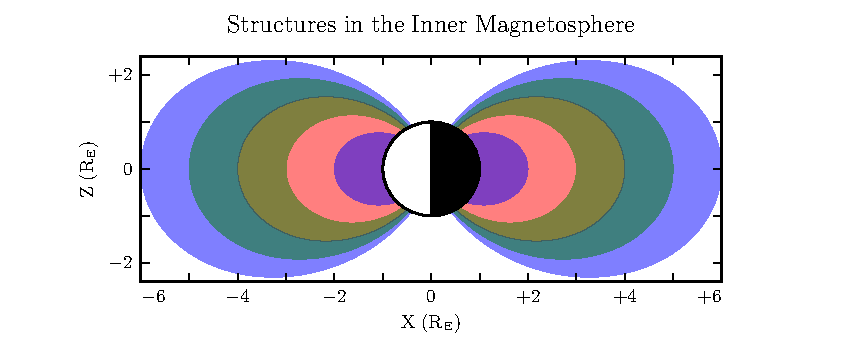
\includegraphics[width=\textwidth]{figures/inner_magnetosphere.pdf}
  \caption[Structures in the Inner Magnetosphere]{
    The above figure shows typical ranges in $L$ for the plasmasphere (red,
    $L < 4$), ring current (green, $3 < L < 5$) and radiation belts (blue,
    $L < 2$ and $4 < L < 6$). These values, particularly the size of the
    plasmasphere, can vary significantly in response to geomagnetic activity. 
  }
  \label{fig_inner_magnetosphere}
\end{figure}

The plasmasphere --- a cold (\about\SI{1}{\eV}), dense
(\SIrange{e2}{e4}{\percc}) torus of corotating plasma --- is formed by the
outward drift of atmospheric ions along magnetic closed field lines. Its outer
boundary is thought to represent a balance between the corotation electric
field (per the rotation of Earth's magnetic dipole) and the convection electric
field (associated with the convection of magnetic flux during the Dungey
cycle). Particle density drops sharply at the edge of the plasmasphere; the
boundary is called the plasmapause. The plasmapause typically falls around
$L=4$, though during prolonged quiet times it can extend to $L=6$ or larger. 

Energetic particles trapped within the inner magnetosphere are divided into two
populations. 

The Van Allen radiation belts are made up of particles with energy above
\SI{e5}{\eV} or so. The inner belt ($L\lesssim2$) is primarily composed of
protons, the decay remnants of neutrons freed from the atmosphere by cosmic
rays. The outer belt ($L\gtrsim4$) is primarily composed of high-energy
electrons. The density of radiation belt particles is significantly affected by
geomagnetic storms and substorms; a typical value is \SI{10}{\percc}. 

Particles with energies of \SIrange{e3}{e5}{\eV} make up the ring current,
which extends from $L\sim3$ to $L\sim5$. Gradient-curvature drift carries ions
and electrons in opposite directions; the net result is a westward current.
During quiet times, the ring current causes magnetic a southward magnetic field
on the order of \SI{1}{\nT} at Earth's equator, while during geomagnetically
active times (discussed in \cref{sec_storms}) the effect may be \SI{100}{\nT}
or more\footnote{For comparison, Earth's dipole field points north at the
equator with a magnitude over \SI{e4}{\nT}. }. 

% -----------------------------------------------------------------------------
% -----------------------------------------------------------------------------
% -----------------------------------------------------------------------------
\section{The Ionosphere}
  \label{sec_ionos}

Earth's neutral atmosphere is an excellent insulator. Collisions are so
frequent that charged particles quickly thermalize and recombine. The breakdown
of air molecules into a conductive plasma (as happens during a lightning
strike, for example) requires electric fields on the order of \SI{e9}{\mV/\m}. 

Cold particles in the magnetosphere are likewise not conducive to currents. In
the absence of collisions, electrons and ions drift alongside one another in
response to an electric field, creating no net current perpendicular to the
magnetic field\footnote{The so-called $E$-cross-$B$ drift is associated with a
velocity of $\vec{U} = \frac{1}{B^2} \vec{E} \times \vec{B}$, independent of a
charged particle's mass or sign. }. Magnetic field lines can typically be
considered as equipotential contours, devoid of field-aligned potential
structures. 

The ionosphere is a sweet spot between the two regimes. Collisions are frequent
enough to disrupt the drift of ions, but not frequent enough to immobilize the
electrons. The result is a finite-valued conductivity tensor. Pedersen currents
(which scale with the Pedersen conductivity) flow in the direction of the
perpendicular electric field. Hall currents (due to the Hall conductivity) flow
in the $\vec{B} \times \vec{E}$. It is these currents --- particularly the Hall
current --- which give rise to magnetic fields at the ground. Collisions in the
ionosphere also result in a finite parallel conductivity, allowing for the
formation of potential structures along the magnetic field line. 

%\todo{Field-aligned currents depend on the level of geomagnetic activity... but do they ever completely go away? }

The convection electric field (associated with the Dungey cycle,
\cref{sec_outer}) drives Pedersen currents in the ionosphere. Pedersen currents
flow dawnward on the flanks and duskward across the poles. The currents remain
divergence-free by connecting to field-aligned currents at the edges of the
polar cap. The field-aligned currents, in turn, connect to the magnetopause
current, the cross-tail current, and the (partial) ring current. 

When electron density is low, thermal velocities may be unable to carry enough
current to satisfy $\nabla \cdot \vec{J} = 0$. This leads to the formation of
potential structures along geomagnetic field lines in the ionosphere. Such
structures accelerate particles along magnetic field lines, leading to the
precipitation of energetic particles into the atmosphere. As the particles
thermalize, they excite atmospheric atoms. The resulting spontaneous emission
is often in the visible spectrum, giving rise to the aurora. 

%\todo{Particles can also be excited by \Alfven waves... this probably goes in \cref{ch_flrs}. }

%From \cite{paschmann_2003}: ``In the thermosphere, the solar ultraviolet (UV) light and energetic particles precipitating from the magnetosphere produce ionization increasing with altitude. At the same time the particle density is low enough to make the recombination times of the ionized atoms and molecules sufficiently long to allow a significant fraction of the gas to remain ionized. This produces a conducting layer of the atmosphere known as the ionosphere. The ionosphere begins at $\sim\SI{65}{\km}$, has a peak plasma density between 200 and 300 km, and eventually merges with magnetospheric regions $\sim$1000--2000 km altitudes.''

%The effects of mean molecular mass on conductivity are computed per the usual definitions. 
%\begin{align}
%  \sp &= \displaystyle\sum_s \frac{n_s q_s^2}{m_s} \frac{\nu_s}{\nu_s^2 + \Omega_s^2} &
%  \sh &= -\displaystyle\sum_s \frac{n_s q_s^2}{m_s} \frac{\Omega_s}{\nu_s^2 + \Omega_s^2} &
%  \sz &= \displaystyle\sum_s \frac{n_s q_s^2}{m_s \nu_s}
%\end{align}

% -----------------------------------------------------------------------------
% -----------------------------------------------------------------------------
% -----------------------------------------------------------------------------
\section{Geomagnetic Storms and Substorms}
  \label{sec_storms}

The quiet geomagnetic behavior described above is periodically disturbed by
transient solar phenomena such as corotating interaction regions (CIRs) and
coronal mass ejections (CMEs). CMEs, such as the one that caused the Solar
Storm of 1859 mentioned in \cref{ch_intro}, are bursts of unusually dense solar
wind which are ejected from regions of high magnetic activity on the Sun; they
are most common at the height of the eleven-year solar cycle. CIRs, on the
other hand, occur when a relatively fast region of the solar wind catches up to
an earlier and slower-moving pocket of solar wind, resulting in a pair of
shockwaves. 

During a storm, increased solar wind intensity results in enhanced magnetic
reconnection on the dayside. As the newly-opened field lines are swept
tailward, the convection electric field is strengthened. The plasmasphere ---
the outer boundary of which is set by a balance between the convection electric
field and the (more or less constant) corotation electric field --- sheds its
outer layers\cite{goldstein_2006}. A large number of energetic particles are
also injected into the ring current\cite{mcpherron_1997}. 

The strength of the storm is gauged by the size of the magnetic perturbation
created by the ring current\footnote{The most commonly used storm index is
\DST, which is computed hourly using measurements from several ground
magnetometers near the equator. The Sym-H index, used in \cref{sec_driving}, is
computed once per minute. }. A small storm has a magnitude of
\SIrange{50}{100}{\nT}. Large storms may reach \SIrange{250}{500}{\nT}. The
Carrington Event, mentioned in \cref{ch_intro}, is thought to have exceeded
\SI{1700}{\nT}\cite{tsurutani_2003}. 

The main phase of a storm typically lasts for several hours. Storm recovery ---
the gradual return of the storm index to zero, and the refilling of the
plasmasphere --- lasts several days. Geomagnetic storms occur tens of times per
year at the height of the solar cycle, and just a few times per year otherwise. 

Whereas storms are prompted by large solar wind events on the dayside,
geomagnetic substorms are primarily a nightside occurrence. As flux accumulates
in the tail, magnetic tension builds in the stretched field lines. A substorm
is an impulsive release of that tension. 

%\todo{Phases of a substorm. Definition of a substorm comes from \cite{akasofu_1964}. Revised by \cite{mcpherron_1973_substorms}. }

At substorm onset, a burst of reconnection occurs in the tail. A jet of plasma
is launched Earthward from the reconnection site (and another is launched
tailward, and lost to the solar wind). The Earthward plasma injection injects
particles into the ring current. The outer radiation belt is depleted, then
repopulated. Energetic particles precipitate into the atmosphere, giving rise
to a distinctive sequence of auroral signatures over the course of about an
hour. 

Concurrent with substorm onset, impulsive \Alfven waves are observed with
periods of a minute or two. The precise ordering of events --- whether
reconnection causes the waves, or vice versa, or if they share a common cause
--- remains controversial. 

Each substorm lasts several hours, including the time it takes for the ring
current to return to pre-substorm levels. Several substorms may occur per day
during quiet times. During a storm, substorms become far more frequent; by the
time one has ended, another may have already begun. 

%\todo{test\cite{daglis_1999,goldstein_2006}. }


%The relationship between geomagnetic storms and geomagnetic substorms is not nearly as neat as their names suggest. Storms are not made of substorms (as atoms are made of subatomic particles), nor are they derivative (as suburbs are to urban areas). Substorms are also not ``below'' storms in any sense (as a subceiling, a submarine, or a subwoofer). Rather, substorms are 

%\begin{longtable}{ @{\extracolsep{\fill}} lrrr @{\extracolsep{\fill}} }
%  \caption[Integrated Ionospheric Conductivity]{Integrated Ionospheric Conductivity (\si{\S})}
%  \label{tab_sigma_ionos} \\
%  \toprule
%  & $\Sigma_0$ & $\Sigma_P$ & $\Sigma_H$ \\
%  \midrule
%  \endfirsthead
%  \bottomrule
%  \endlastfoot
%  Active Day   & --- & 13.0 & 17.0 \\
%  Quiet Day    & --- & 5.6  & 10.2 \\
%  Active Night & --- & 0.8  & 0.3 \\
%  Quiet Night  & --- & 0.2  & 0.3 \\
%\end{longtable}


